\documentclass[11pt]{article}
\usepackage{aas_macros}
\usepackage{hyperref}
\usepackage[hmargin=1.5cm, vmargin=0.55cm]{geometry}
\usepackage{amsmath}
\usepackage{caption}
\usepackage{mathtools}
\usepackage{fancyhdr}
\usepackage{float}%Places the float at precisely the location in the LaTeX code...i.e, [H]
\usepackage{wrapfig}
\usepackage[pdftex]{graphicx}%includegraphics
%converts eps to pdf
%\usepackage{subcaption} %need to find subcaption.sty for this to work!
%\usepackage{epstopdf}
\DeclareGraphicsExtensions{.pdf,.png,.jpg,.eps,.gif}
%\graphicspath{{~/PhD/Thesis/Figures/}}

\renewcommand{\vec}[1]{\mathbf{#1}}
\usepackage[round]{natbib}  %use the "Natbib" style for the references in the Bibliography
%\usepackage{aastex}%defines journal abbreviations in bib file
%\newcommand{name}[num]{definition}



\title{Upgrade Report}
\author{Jamie Ryan \\ 
Mullard Space Science Laboratory \\
University College London \\
Surrey, RH13 6NL, UK\\
\href{mailto:jamie.ryan.14@ucl.ac.uk}{jamie.ryan.14@ucl.ac.uk}
\date{}}
\begin{document}
\maketitle
\tableofcontents

%%%%%%%%%%%%%%%%%files containing bodies of text%%%%%%%%%%%%%%%%%%
%%%%%%%%%%%%%%%%%%%%%%%%%%%%%%%%%%%%%%%%%%%%%%%%%%%%%%%%%%%%%%%%%%
%%%%%%%%%%%%%%%%%%%%%%%%%%%%%%%%%%%%%%%%%%%%%%%%%%%%%%%%%%%%%%%%%%
%\begin{abstract}
Sunquakes represent the propagation of acoustic waves in the sub-photosphere, responding to an excitation of the photosphere during the impulsive phase of solar flares. The progenitors of sunquakes are thought to be either shocks, radiative backwarming, direct particle collision or sudden magnetic field reconfiguration. Each of these mechanisms relies on the transport of energy from the corona to the photosphere, and the physical conditions existing in the chromosphere such as magnetic configuration and density. To understand sunquakes and their relationship to solar flares, we need to understand how energy moves down through the solar atmosphere and the physical conditions that are present. An X1 solar flare with associated sunquake was observed in active region NOAA 12017 on the 29th of March 2014 at 17:46 UTC, by multiple spacecraft, including SDO (HMI), IRIS and RHESSI. Lightcurves of the flare emission from the photosphere, chromosphere and transition region are analysed providing information about the deposition of energy at different altitudes in the solar atmosphere. Hard X-ray footpoints of coronal loops are shown to align well with an area associated with maximum acoustic power. Balmer continuum emission aligned with maximum acoustic power is shown to increase during the flare, indicating the existence of hydrogen recombination continua in the chromosphere possibly leading to radiative backwarming of the photosphere. 
\end{abstract}

\section{Sunquakes}
\subsection{Introduction}
%Chronological soft intro; use some of the lit review,
%making sure to emphasize the connection to solar flares;Look at early papers predicting sunquakes(Wolff 70s and Kosovichev and Zharkova);the importance of sunquakes


During this age of space-born solar astronomy, understanding the highly dynamic environment of the Sun's atmosphere is a study enriched by a wealth of high detail observations. With each newly launched space instrument the spatial resolution of collected data increases, which coupled with those spacecraft that are tailored to capture light of previously unobserved wavelengths, often leads to new phenomena being observed. Eruptive solar flares fall into this category, in that spacecraft have provided observations that challenge the current theoretical view that the standard eruptive flare model (CSHK model: \citep{1964NASSP..50..451C, 1966Natur.211..695S, 1974SoPh...34..323H, 1976SoPh...50...85K} puts forward. 

Solar flares are one of the most energetic events to occur in the Sun's atmosphere, where by stored magnetic energy is released in the form of heat, mass motions, and accelerated particles. This highly dynamic process produces many measurable signatures, such as emission from $\gamma$-ray to optical wavelengths, a high percentage of which agree with the CSHK model, however, this is not the full picture. The standard flare model has been modified to include new observations many times over the years \citep{2011LRSP....8....6S} and is still unable to describe some observed phenomena. Therefore there is still work to be done before a true account of the complex nature of solar flares are to be realised.    

Sunquakes are an observable feature during some solar flares that the standard model is unable to explain. It is believed that they are the result of energy and momentum released during the flare impacting the lower solar atmosphere. During a solar flare, energy is released high up in the solar atmosphere and transported down to lower altitudes. If a sufficient amount of energy impacts the lowest atmospheric layer, then acoustic waves are produced which propagate into sub-surface layers of the Sun observed on the solar surface as a sunquake (see Figure \ref{sunquake-cartoon}a). As acoustic wave-fronts travel into the interior they encounter layers of increasing density causing refraction back toward the solar surface (see Figure \ref{sunquake-cartoon}b). At which point, waves can be observed as circular formations in the surface plasma, expanding outward from a point of origin (see Figure \ref{mdiquake96}). 


\begin{figure}[hb]%\label{sunquake-cartoon}
  \begin{center}
  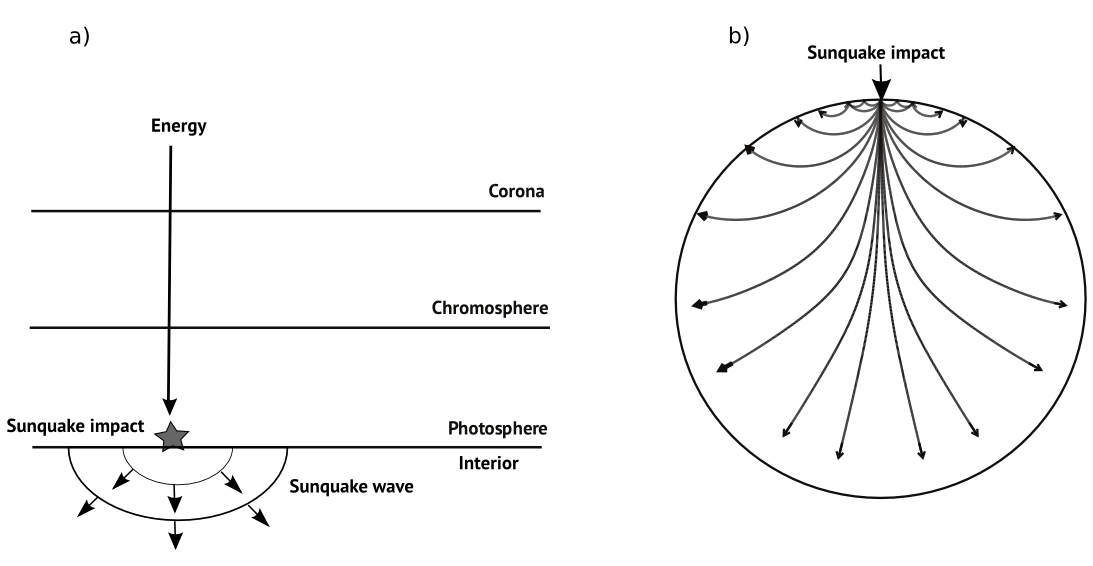
\includegraphics[width=0.99\textwidth]{sunquake-cartoon}
  \caption{Sunquake cartoon: a) Shows a basic picture of sunquake production. Energy moves down through the solar atmosphere impacting the photosphere and generating a sunquake. b) Shows acoustic wave-fronts propagating into the interior of the Sun. Wave-fronts refract back toward the surface as they encounter increasingly dense sub-surface layers. Waves reaching the surface disturb material in a pattern resembling ripples in a pond.}\label{sunquake-cartoon}
\end{center}
\end{figure}

\subsection{Sunquake Observations}
The idea that solar flares can cause acoustic waves inside the Sun was originally put forward by \citep{1972ApJ...176..833W}. Wolff made the connection that a large solar flare releasing enough energy to heat the photosphere, would generate expansion of photospheric material, which could lead to an impulsive stimulation of oscillations in the Sun's interior. Wolff also commented that it would be difficult to observe interior oscillations with current (in the 1970s) solar velocity measurement techniques.      

A little over twenty years later and Wolff's idea was built upon by \cite{1995ESASP.376b.341K}, who showed theoretically that acoustic waves in the solar interior could be generated by a large solar flare, and that they may be detectable. A year later and the first detection of a sunquake was made by \cite{1998Natur.393..317K} during an X class solar flare on July the 9th 1996. Their observational data came from the Solar and Heliospheric Observatory (SOHO) via the Michelson Doppler Imager (MDI) which images the movement of photospheric material by analysing shifts in wavelength of the emitted light. They observed a prominent impulsive downward signature in the Dopplergrams directly over a compact point source which subsequently emanates a set of concentric acoustic waves (see Figure \ref{mdiquake96}). The timing of maximum downward velocity of material derived from the Dopplergrams was out of sync with peak hard x-ray measurements by around a minute. This time delay, coupled with white-light enhancement in the lower atmosphere led to the conclusion that during the flare, accelerated energetic particles heat the cool dense chromosphere causing a shock front which travels downward, depositing energy in lower atmospheric layers, generating a sunquake. 
 
\begin{figure}[hb]
  \begin{center}
  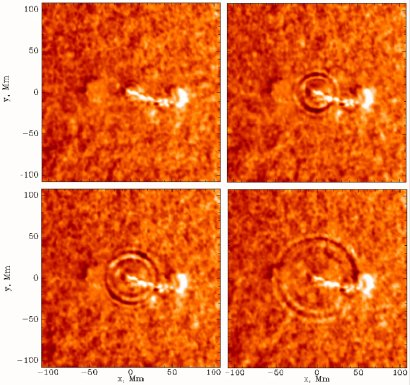
\includegraphics[width=0.80\textwidth]{soho-mdi-quake-96}  
\caption{\cite{1998Natur.393..317K} produced SOHO MDI Dopplergrams from the 1996 July 9th, X class solar flare showing the sunquake expanding outward from it's seismic epicentre to a radial distance of $1.2\times10^{8}$ metres. Wave-fronts accelerate from a velocity of 30km/s to 100km/s}\label{mdiquake96}
\end{center}
\end{figure}


The first sunquake observation opened up a whole new area of solar physics, leading to a multitude of detections associated with many different flares. The majority of observations show that sunquakes are often the product of highly impulsive flares, with the acoustic source aligning spatially with white light enhancement in the lower solar atmosphere and hard x-ray emission in the upper-atmosphere \citep{2005ApJ...630.1168D, 2007ApJ...664..573Z}. \cite{2005ApJ...630.1168D} went on to calculate the energy needed to stimulate the propagation of an acoustic wave in the sub-photosphere, finding that only $\sim10^{-3}$ of the energy released by a flare is enough to generate a sunquake. This was an important calculation because it forced the solar community to consider that it might be possible for low energy flares to produce sunquakes, leading subsequent work by \cite{2008SoPh..251..613M} looking at seismicity of M-class flares.

A paper by \cite{2000ApJ...531L..75H} put forward for the first time, that sunquake production may depend on the changing configuration of the local magnetic field. This idea was further reinforced by \cite{2001ApJ...550L.105K} reporting observations of impulsive changes in magnetic field strength at the photosphere during a solar flare. These magnetic transients were shown to approximately correlate in time and space with hard x-rays, impulsive increases in plasma velocity and increased emission. This line of study was continued \citep{2009MNRAS.395L..39M}, investigating the magnetic field variation of the photosphere in many flares. The study found that some flares with seismicity do not have a spatial and temporal correlation between sunquakes and magnetic transients. Some flares have magnetic transients and no seismicity, and some flares have a good co-spatial alignment of acoustic activity and magnetic variability. It was noted that the impulsiveness of the magnetic field variation could be important as to whether a sunquake is generated.

Some of the most intriguing of sunquake observations are those that do not abide by the usual set of observable features, in that they are not necessarily associated with hard x-rays and excess white-light emission. For example, a statistical survey carried out by \cite{2012SoPh..277..317P}, highlighted a flare containing three footpoints with a seismic source that was co-temporal but not co-spatial with it's closest HXR footpoint; and another source which was co-spatial and co-temporal with it's nearest HXR footpoint. Showing that a sunquake does not necessarily have to be directly under locations of peak emission. Another example by \cite{2011ApJ...741L..35Z} reports an observation of two seismic sources associated with footpoints of an erupting flux rope. During the eruption, the magnetic field above each seismic source undergoes an abrupt permanent reconfiguration. The authors cite the possibility that there exists particle beams low enough in population that HXR emission is undetectable. Further papers investigating the same event \citep{2013SoPh..284..315Z} show that there are downward motions of material above the seismic sources and that energy provided by magnetic transients may not be able to account for the acoustic power generated. These observational oddities prove that mechanisms that generate sunquakes are not well understood and there is much research to be done to classify the different progenitors.      

\subsubsection{Sunquake Progenitors}\label{sunprog}
%list and explain current theories of sunquake generation
%making sure to highlight the different observables that can identify each mechanism, eg wlf = evidence of radiative backwarming  


The progenitors of sunquakes are still unknown and as a result this is an exciting area of research with discoveries still to be made. The general consensus, in terms of valid mechanisms that could cause this phenomenon is an area of contention, however the following progenitors are thought to be at least partly responsible. \\

\begin{itemize}
\item \textbf{Radiative backwarming} as a mechanism for producing sunquakes, was first put forward by \cite{2005ApJ...630.1168D} to account for a spatial correlation between seismic sources and white light emission from the lower atmosphere. During a solar flare, high energy electrons and photons impulsively heat the lower chromo or photosphere producing an enhancement in white light emission \citep{1989SoPh..124..303M}. This causes an impulsive increase in radiation pressure and gas pressure exerted on the photosphere, generating acoustic waves which propagate into the sub-photosphere. \\
     
\item \textbf{Sudden magnetic field reconfiguration} was first detailed by \cite{2008ASPC..383..221H}. Solar flares are violent physical processes that involve the evolution of magnetic fields and charged solar plasma. Due to the Lorentz force, it is possible for a magnetic field to impart a force on a charged material and vice versa. If, during a solar flare, the magnetic field close to the photosphere relaxes to a more horizontal alignment it can impart a force on the photospheric material resulting in the production of acoustic waves, which propagate into sub-photosphere. The key parameter for this mechanism seems to be that the field has to reconfigure in an sufficiently impulsive manner to generate enough force to induce seismic waves. \\

\item \textbf{Shocks} are a mechanism originally proposed in initial work by \cite{1995ESASP.376b.341K} and \cite{1998Natur.393..317K}, whereby a shock wave propagates from the upper-chromosphere down to lower altitudes. During a solar flare, particles and heat are directed down toward the chromosphere, at which point chromospheric material reacts by increasing in temperature. This increased temperature causes explosive ablation of chromospheric material both upward and downward. The downward component develops into a shock front carrying energy to the lower atmosphere, which can go on to impact the photosphere generating acoustic waves. If the shock is dissapated at higher altitudes such as the lower chromosphere, heat generated during the deposition process can irradiate the photosphere with high energy photons, causing radiative backwarming \citep{1989SoPh..124..303M}. \\

\item \textbf{Direct proton collision}, is linked to observations by \cite{2007ApJ...664..573Z} where the sunquake was spatially aligned with $\gamma$-ray emission. $\gamma$-rays during a solar flare are an indicator of energetic protons being accelerated along a newly reconfigured magnetic field. Proton beams carry more momentum than electron beams and are able to penetrate through the chromosphere to lower atmosphere. If an energetic beam of protons makes it down to the photosphere, it can deposit energy in the form of an impact, which due to conservation of momentum will generate acoustic waves in the sub-photosphere. \\

\end{itemize}

\section{Eruptive Solar Flares}
\subsection{An Introduction to the Standard Eruptive Flare Model} 

Solar flares are the manifestation of magnetic energy release in the form of electromagnetic radiation spanning a wide range of wavelengths. These events are the most energetic phenomena associated with the Sun, with some of the larger flares releasing $10^{37}$ erg of energy. Flares are classified by the X-ray flux measured by the Geostationary Operational Environmental Satellite (GOES) see Table \ref{goes} below. \\

\begin{table}[h]
\centering
\begin{tabular}{|c|c|}\label{GOES}
Classification & Peak Flux Range at 1 to 8 \AA\ ($W.m^{-2}$)\\ 
\hline
X & $10^{-3}$ - $10^{-4}$\\ 
M & $10^{-4}$ - $10^{-5}$\\ 
C & $10^{-5}$ - $10^{-6}$\\ 
B & $10^{-6}$ - $10^{-7}$\\ 
A & $<10^{-7}$\\  
\end{tabular}
\caption{shows the GOES flare classification, which is based on powers of ten of hard x-ray flux. X class flares are the most powerful and A class are the weakest.}\label{goes}
\end{table}

The exact physical process governing the mechanics of solar flares is not known, however, magnetic reconnection is the currently accepted mechanism. Coronal magnetic loops tethered to sunspots of opposing polarity in the photosphere and sub-photosphere are twisted and stressed by movements of active regions across the solar surface. This shearing of the magnetic field, effectively stores energy as magnetic tension which can be released when opposing field lines meet and reconnect. The process of energy conversion is basically an unstable tensioned magnetic field relaxing back to a more stable configuration. As a result stored magnetic energy is converted to radiation, kinetic and thermal energy. The standard 2D flare model is the culmination of research by many authors,\citep{1964NASSP..50..451C, 1966Natur.211..695S, 1974SoPh...34..323H, 1976SoPh...50...85K}, and is still an ongoing area of research that is not entirely understood \citep{2011LRSP....8....6S}. In an active region, a closed magnetic field harbouring a flux rope suddenly opens. As a result, plasma flows from the chromosphere to the corona. Because material in the chromosphere is denser than in the corona, flowing plasma experiences a drop in plasma pressure and an increase in magnetic pressure. This leads to reconnection of the open magnetic field lines, forming new loops at lower altitudes. Reconnection causes excess heating at the peaks of newly connected loops which conducts down toward the chromosphere. Also, particles are accelerated by the new magnetic configuration, flowing to the chromosphere. This injection of thermal energy and accelerated particles heats the chromosphere causing HXR footpoints \citep{1995ApJ...455..347A} and UV ribbons \citep{2009A&A...493..241F}. As a result, some chromospheric material evaporates upward into newly created flare loops, whilst some material propagates downward toward the lower chromosphere. The flare loop cools and the process starts again in the next consecutive loop until the unstable magnetic field has relaxed to a state that is closer to it's stable,  potential state. In eruptive flares, energy is released every time a new reconnection of a neighbouring loop occurs, this is the reason that flare ribbons appear move away from each other as the flare evolves. \\
White light flares are said to be rare events only associated with the most energetic of solar flares, they occur when flare energy is transported deep into the dense lower atmosphere causing an enhancement in optical wavelengths. It is thought this happens due to an energetic particle beam transporting energy to the lower atmosphere where it's energy dissipates into the dense chromospheric or photospheric material. The collisional thick target model by \cite{1971SoPh...18..489B} says that almost all of the flare energy is carried by the particle beam, therefore, energy dissipated in the lower atmosphere represents a large portion of the flare energy budget. White light enhancement from the lower atmosphere can be explained by either, Balmer \& Paschen continuum emission from the chromosphere caused by hydrogen recombination or direct photospheric heating \citep{2007ASPC..368..417D} by radiative backwarming \citep{1989SoPh..124..303M}. 


\begin{figure}[H]
  \begin{center}
  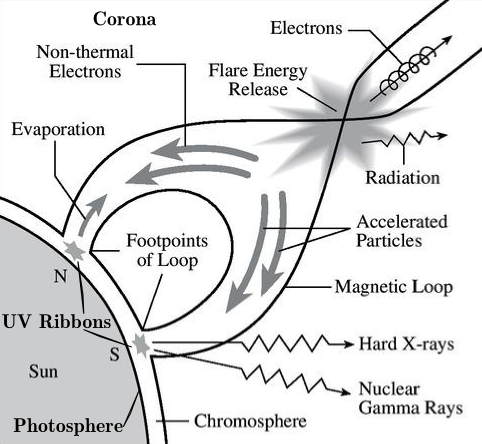
\includegraphics[width=0.40\textwidth]{flare}
  \caption{cartoon of the standard 2D solar flare model.}\label{flare-cartoon}
\end{center}
\end{figure}


%It is also theoretically possible to heat the upper photosphere by resistive dissipation of Alfven waves \citep{1982SoPh...80...99E}


\subsubsection{Solar Atmosphere}
The solar atmosphere is described as having four main components, the corona, transition region, chromosphere and photosphere, see Figure \ref{solatmpics}. 

\begin{figure}[H]%\label{sunquake-cartoon}
  \begin{center}
  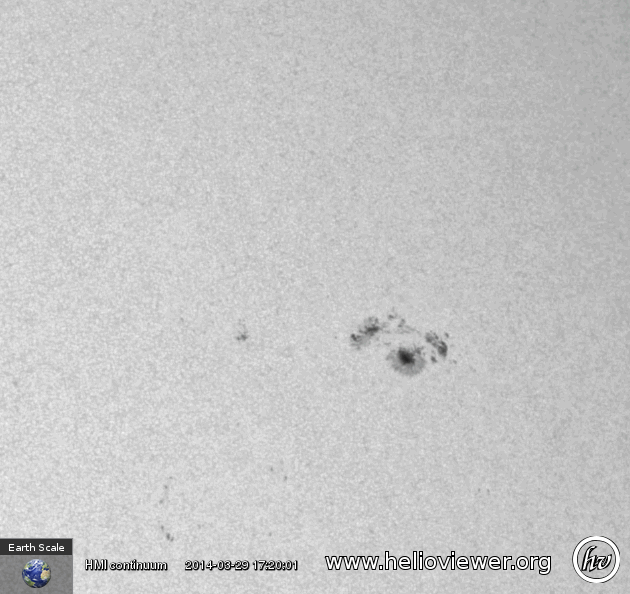
\includegraphics[width=0.20\textwidth]{2014_03_29_17_19_42_HMI_Int}%photsphere
  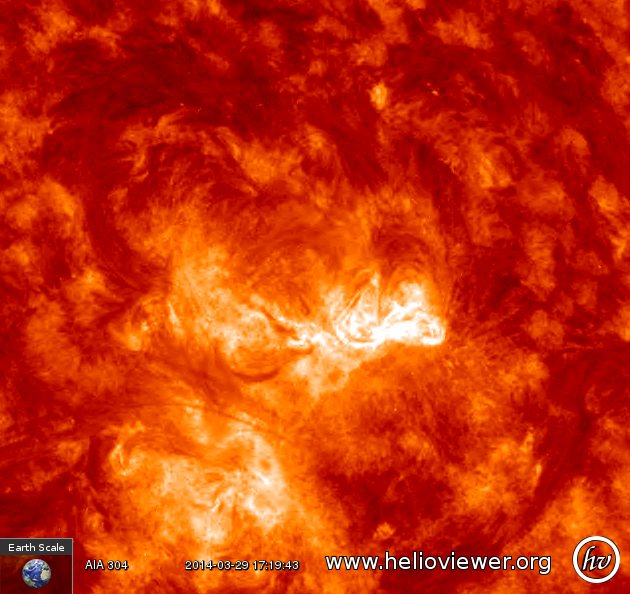
\includegraphics[width=0.20\textwidth]{2014_03_29_17_19_42_AIA_304}%chromosphere
  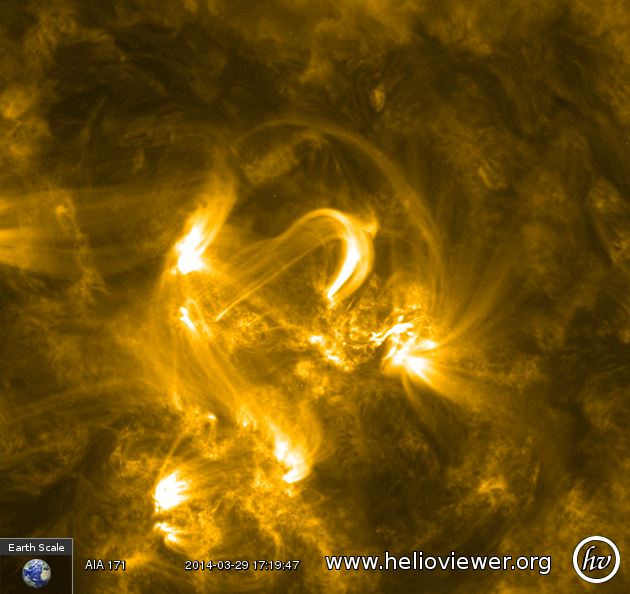
\includegraphics[width=0.20\textwidth]{2014_03_29_17_19_42_AIA_171}%tr
  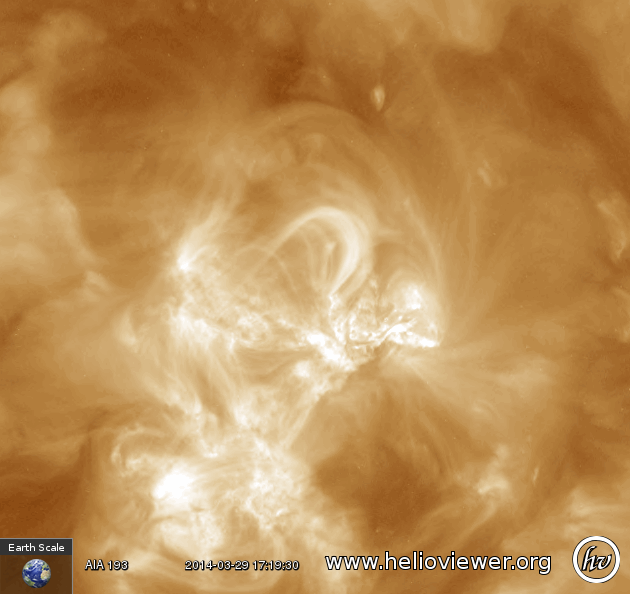
\includegraphics[width=0.20\textwidth]{2014_03_29_17_19_42_AIA_193}%corona
  \caption{ Images taken from the Solar Dynamics Observatory (SDO) instruments, the Helioseismic Magnetic Imager(HMI) and the Atmospheric Imaging Assembly (AIA) displaying the four main components of the solar atmosphere. From left to right layers of the solar atmosphere are increasing in altitude and temperature from the photosphere (SDO/HMI 6173 \AA\ continuum), to the chromosphere (SDO/AIA 304 \AA) through the transition region (SDO/AIA 171 \AA) then up to the corona (SDO/AIA 193 \AA).}\label{solatmpics}
\end{center}
\end{figure}


For a sunquake to occur, energy released during a solar flare has to traverse these four layers propagating through nine pressure scale heights as it does so. Pressure scale height is a measure of the distance over which pressure drops off by a factor of $\exp$, for example, in the photosphere, $H\sim150$km, whereas in the corona, $H\sim100$Mm. The photosphere is where sunquakes form observable wave-fronts and is the lowest in altitude of the four layers. With an effective temperature of $T=5800$K, the photosphere decreases in temperature with radial distance. If white light enhancement is observed in the photosphere, it is thought to be an indicator of the \textbf{Radiative backwarming} progenitor of sunquake generation, which can also be a bi-product caused by chromospheric \textbf{Shocks}. The plasma beta (a measure of the ratio between gas and magnetic pressure) in this region is mostly larger than one $\beta >1$ meaning plasma pressure is dominant in dictating plasma motions, the exception to this exists in sunspots where $\beta<1$ and magnetic pressure is dominant. \\ 

Found in active regions of the photosphere, sunspots are regions of intense magnetic field playing host to footpoints of loops that can extend out into interplanetary space. They are made up of two main parts, the dark central umbra, surrounded by the slightly less dark penumbra. The umbra hosts magnetic field lines that are tightly packed and pointing radially away from the Sun, whereas the penumbral magnetic field is more horizontal with respect to the solar surface. During a solar flare, coronal loops reconnect causing a reconfiguration of the magnetic field tethered at sunspot locations, at this point, penumbral field lines can collapse toward the photosphere, imparting a Lorentz force on local plasma. This leads to the \textbf{Sudden magnetic field reconfiguration} progenitor of sunquake generation. Other features that are found on the photosphere include granules, which are the physical representation of convection currents. Heated plasma rises from below the surface and is seen as the bright central part of the granule, the darker surrounding regions are cooler material sinking back into the interior. \\

The next region of the atmosphere is the chromosphere which is situated above the photosphere. This layer of plasma is a few thousand kilometres (2000-3000km) thick and is optically thin to visible light so is difficult to see against the brightness of the photosphere. The temperature in this layer increases with height and ranges from 4400K at the temperature minimum region to $\sim10^{5}$K at the top, as a result, $\beta$ drops rapidly crossing unity as it does so. The pressure scale height in this region is changing with altitude. Through the transition region to the corona and the atmosphere starts to heat considerably to $T\sim10^{7}$K. This region is visible in white light due to Thompson scattering of photospheric light by free electrons and dust in the coronal magnetic field. The plasma beta is less than one through the entire corona meaning magnetic forces dominate. Figure \ref{solatm} shows how the solar atmosphere changes with height, temperature and density, giving an indication of the stratification of atmospheric layers. Information in this section is taken from text books: \cite{2003dysu.book.....D, 2004soas.book.....F}

\begin{figure}[H]
  \begin{center}
    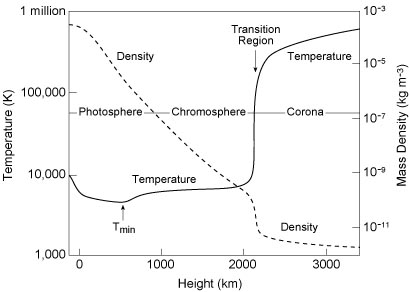
\includegraphics[width=0.6\textwidth]{solar-atm-plot}
\caption{The temperature of the solar atmosphere decreases from values near 6,000 degrees Kelvin at the visible photosphere to a minimum value of roughly 4,400 degrees Kelvin about 500 kilometres higher up. The temperature increases with height, slowly at first, then extremely rapidly in the narrow transition region, less than 100 kilometres thick, between the chromosphere and corona, from about $10^{4}$K to about $10^{6}$K. (Courtesy of Eugene Avrett, Smithsonian Astrophysical Observatory.)}\label{solatm}
  \end{center}
\end{figure}

  
\subsection{Observing Solar Flares}
Using data collected by spacecraft observing the Sun, energy released during solar flares can be tracked as it is deposited throughout the atmosphere. Energy deposition in the corona and upper chromosphere is marked by HXR footpoints and UV ribbons. The Ramaty High Energy Solar Spectroscopic Imager (RHESSI) observes solar emission ranging from X-rays to $\gamma$-rays produced by energetic particles and nuclear interactions. RHESSI was designed with the aim of understanding impulsive energy release, particle acceleration and transportation in the magnetohydrodynamic environment of the solar atmosphere. Using 25 - 50 keV and 50 - 100 keV intensity data collected by RHESSI, HXR footpoints can be tracked and analysed. \\
Observing UV ribbons requires a different spacecraft. The Interface Region Spectroscopic Imager (IRIS) captures near-ultraviolet (NUV) and far-ultraviolet (FUV) emission and is designed to observe the chromosphere at various altitudes. Emission is collected by a slit-jaw imager (SJI) and a spectrometer (SG) simultaneously. The spectrograph is sensitive in both FUV and NUV passbands, which expose 3 CCDs to produce spectra in three UV bands, two FUV and one NUV. Table \ref{iris-sg} shows how each passband relates to emission processes occurring from the upper-chromosphere down to the upper-photosphere. 

\begin{table}[H]
\centering
\begin{tabular}{|c|c|c|c|}
Band & Wavelength \AA\ & Temperature $\log{T}$ & Region of Atmosphere\\ 
\hline
FUV 1 & $1331.7 - 1358.4$ & $3.7 - 7.0$ & Upper to lower-chromosphere\\ 
FUV 2 & $1389.0 - 1407.0$ & $3.7 - 5.2$ & Upper to lower-chromosphere\\ 
NUV & $2782.7 - 2851.1$ & $3.7 - 4.2$ & Chromosphere to upper-photosphere\\ 
\end{tabular}
\caption{The IRIS/SG is capable of observing three passbands, which relate to different plasma temperatures.}\label{iris-sg}
\end{table}

The slit-jaw images, are light collected from a reflective area surrounding the slit. The imager is capable of observing four wavelengths relating to emission at different altitudes as shown by Table \ref{iris-sj}. 

\begin{table}[H]
\centering
\begin{tabular}{|c|c|c|c|c|}
SJI Passband & Wavelength \AA\ & FWHM \AA\ & Temperature $\log{T}$ & Region of Atmosphere\\ 
\hline
C II  & $1330$ & $40$ & $3.7 - 7.0$ & Upper-chromosphere\\ 
Si IV  & $1400$ & $40$ & $3.7 - 5.2$ & Upper-chromosphere\\ 
Mg II h/k & $2796$ & $4$ & $3.7 - 4.2$ & Lower-chromosphere\\ 
Mg II wing & $2832$ & $4$ & $3.7 - 3.8$ & Upper-photosphere\\   
\end{tabular}
\caption{The IRIS/SJ is capable of observing four passbands, which relate to different plasma temperatures.}\label{iris-sj}
\end{table}  

Signatures from energy deposition in the lowest regions of atmosphere are captured by Solar Dynamics Observatory's (SDO) Helioseismic Imager (HMI), which observes the photosphere. Able to observe optical continuum intensity (6173 \AA), helioseismic and magnetic data, SDO/HMI can provide valuable insight into WLFs, sunquakes and magnetic field configuration. Optical continuum data can provide information about WLFs and radiative backwarming of photospheric material, which is a possible sunquake progenitor. Helioseismic data can be used to analyse the movement of material during a solar flare, such as downward flows which could indicate shocks propagating from higher altitudes or particle beams penetrating the atmosphere. The point of origin and wave-fronts of a sunquake can also be detected using helioseismic data, which can be used to calculate acoustic power of the quake. Magnetic data from SDO/HMI shows local magnetic field direction, useful for determining the presence of impulsive changes in magnetic field capable of generating a sunquake.     



%%%%%%%%%%%Observable Seismic Signatures%%%%%%%%%%%%%%%%%%%%%%%%%%
\subsection{Observable Seismic Signatures}
%Basics of helioseismology and challenges of observing acoustic emission
Helioseismology is a tool for probing the interior of the Sun. Most techniques in this field of analysis rely on observations of gravity and acoustic waves on the photosphere that are the result of interior excitation. Studying the frequency and modes of these oscillations has revealed much about the internal structure of the Sun. Local helioseismology is a collection of techniques developed for global helioseismology that have been modified for use in studying local regions in higher spatial resolution. The following section provides a very basic introduction to some of these techniques. 

\subsubsection{Local Helioseismology}
%use content from old report...maybe expand a little

\paragraph{Helioseismic Holography}\label{helioholog}
\cite{1999ApJ...513L.143D} pioneered the use of helioseismic holography to produce seismic images of the solar flare of July 1996 reported to have a sunquake by Kosovichev and Zharkova. Time series egression-power maps at 3.5 and 6 mHz were computed with a 2 mHz bandwidth. It was found that the most powerful acoustic power frequency associated with the flare is centred at 3.5 mHz but has a large signal to noise ratio. Whereas the 6 mHz range has a much lower ambient noise, therefore producing a better rendering of the seismicity of the flare. It is now standard practice to use the 6 mHz range for helioseismic holographic calculations of egression-power. \\
Originally the idea of analysing Doppler images of the solar surface in order to observe acoustic sources was put forward by \cite{1975CRASB.281...93R}. Helioseismic holography was developed further in concept by Lindsey and Braun \citep{1990SoPh..126..101L, 1992ApJ...392..739B, 1997ApJ...485..895L} in an effort to to image the solar interior and far-side of the Sun. This technique involves using a Doppler image as a representation of the wave-field at a location on the solar surface as a reference point to be able to estimate that wave-field a location in the solar interior at a time preceding or proceeding the image. This is achieved by calculating the ingression or egression of the wave-field by assuming that it's evolution is a, convergence to, or divergence from, the point of origin of that wave-field. 
This technique uses Green's function (eqn \ref{green}, where $\vec{r}$ and $t$ are position and time of an observed signal and $\vec{r}'$ and $t$' are the position and time of the signal earlier in time) which assumes the that the acoustic wave propagates from a point source, allowing a signal $\psi(\vec{r},t)$ observed on the surface to be devolved backwards in time. 

\begin{equation}\label{green}
G_{+}(|\vec{r}-\vec{r}'|,t-t')
\end{equation}

Where $a$ and $b$ constrain the holographic pupil, equation \ref{holog} is then used to devolve the surface signal to calculate the position of subsurface acoustic sources. 

\begin{equation}\label{holog}
H_{+}(\vec{r},z,t)= \int dt'  \int_{a<|\vec{r}-\vec{r}'|<b} d^{2}\vec{r}'G_{+}(|\vec{r}-\vec{r}'|,t-t')\psi(\vec{r}',t')
\end{equation}

Equation \ref{eggpower} is then used to calculate the egression power associated with the acoustic sources at a time $t$. 

\begin{equation}\label{eggpower}
P(z,\vec{r})=\int dt|H_{+}(\vec{r},z,t)|^{2}dt
\end{equation}

If egression power is required in terms of frequency then equation \ref{eggpower} can be Fourier transformed into frequency space.


\paragraph{Time-Distance}\label{TD}
The first observation of a sunquake \citep{1998Natur.393..317K} used the time-distance technique to track sunquake wavefronts. The paper by \cite{1993Natur.362..430D} explains how to extract time-distance (TD) information from observations of intensity fluctuations on the solar surface. This technique uses travel times of waves between two locations on the solar surface. The method assumes that the travel time of a wave propagating in the interior of the Sun will be modified by any anomalies that it has to travel through, thus the resulting signal will contain the signatures of those irregularities. For instance, if the wave encounters a flow along it's path of travel, it will propagate faster with the flow than against it, affecting travel time.     
This technique remaps Dopplergrams into polar coordinates, with the point of origin centred on the area of downflowing material during the flare. This remapped image is then Fourier transformed with respect to azimuthal angle, with the resulting image highlighting circular disturbances as a line of positive slope.    

%\subsection{Sunquake Model}
%Intro to the physics of sunquakes + cartoon


%%%%%%%%%%%%%%%%%%%%%%%%%%%%%%%%%%%%%%%%%%%%%%%%%%%%%%%%%%%%%%%%%%%%%%%%%%%%%%%%%%%%%%%%%%
%%%%%%%%%%%Progenitors of sunquakes%%%%%%%%%%%%%%%%%%%%%%%
\subsubsection{Sunquake Progenitors}\label{sunprog}
%list and explain current theories of sunquake generation
%making sure to highlight the different observables that can identify each mechanism, eg wlf = evidence of radiative backwarming  


The progenitors of sunquakes are still unknown and as a result this is an exciting area of research with discoveries still to be made. The general consensus, in terms of valid mechanisms that could cause this phenomenon is an area of contention, however the following progenitors are thought to be at least partly responsible. \\

\begin{itemize}
\item \textbf{Radiative backwarming} as a mechanism for producing sunquakes, was first put forward by \cite{2005ApJ...630.1168D} to account for a spatial correlation between seismic sources and white light emission from the lower atmosphere. The idea is that during a solar flare, high energy electrons and photons impulsively heat the photosphere producing white light emission \citep{1989SoPh..124..303M}. This causes an increase in radiation pressure in the photosphere which causes acoustic waves to propagate into the sub-photosphere. \\
     
\item \textbf{Sudden magnetic field reconfiguration} was first detailed by \cite{2008ASPC..383..221H}. Solar flares are violent physical processes that involve the evolution of magnetic fields and charged solar plasma. Due to the Lorentz force, it is possible for a magnetic field to impart a force on a charged material and vice versa. If, during a solar flare, the magnetic field close to the photosphere relaxes to a more horizontal alignment it can impart a force on the photospheric material resulting in the production of acoustic waves, which propagate into sub-photosphere. Thekey parameter for this mechanism seems to be that the field has to reconfigure in an sufficiently impulsive manner to generate enough force to induce seismic waves. \\

\item \textbf{Shocks} are a mechanism originally proposed in initial work by \cite{1995ESASP.376b.341K} and \cite{1998Natur.393..317K}, whereby a shock wave propagates from the upper-chromosphere down to the photosphere generating sub-photospheric acoustic waves. During a solar flare, particles and heat are directed down toward the chromosphere, at which point chromospheric material reacts with and increase in temperature. This increased temperature causes explosive ablation of chromospheric material both upward and downward. The downward component develops into a shock front carrying energy to the lower atmosphere, which can go on to heat the photosphere causing radiative backwarming \citep{1989SoPh..124..303M}. \\

\item \textbf{Direct proton collision}, is linked to observations by \cite{2007ApJ...664..573Z} where the sunquake was spatially aligned with $\gamma$-ray emission. $\gamma$-rays during a solar flare are an indicator of energetic protons being accelerated along a newly reconfigured magnetic field. Proton beams carry more momentum than electron beams and are able to penetrate into the lower atmosphere, depositing energy in the form of heat. If an energetic beam of protons makes it down to the photosphere, it can cause radiative backwarming \citep{1989SoPh..124..303M}, which in turn causes the sunquake as described above. \\

\end{itemize}





%\section{Eruptive Solar Flares}
\subsection{An Introduction to the Standard Eruptive Flare Model} 
standard solar flare model
cartoon
\subsection{Observing Solar Flares}
a bit about the the spacecraft and instrumentation providing the data for my research. Make sure to explain abbreviations
\subsubsection{Solar Atmosphere}
a bit about observing different layers of the atmosphere in different wavelengths...how do we know the altitudes of the emission?
can use modified solar atmosphere section (from old report)....rewrite pressure scale height...i.e,energy moving through the atmosphere has to traverse 9 pressure scale heights...what that means
\subsection{Magnetohydrodynamics of Solar Flares}
mhd maths and explanation..and what the induction equation physically means...maybe use a figure!!!
get to grips with the derivation, why is each assumption made?
can use mhd section from old report



%%%%%%%%%%%%%%%%%%%%%%%%%%%%%%%%%%%%%%%%%%%%%%%%%%%%%%%%%%%%%%%%%%%%
%old report content

%%%%%%%%%%%%%%%%%%%%%%Eruptive Flare Model%%%%%%%%%%%%%%%%%%%%%%%%%%
\subsection{Eruptive Flare Model}\label{EFM}
Solar flares are the manifestation of magnetic energy release in the form of electromagnetic radiation spanning a wide range of wavelengths. These events are the most energetic phenomena associated with the Sun, with some of the larger flares releasing $10^{37}$ erg of energy. Flares are classified by the X-ray flux measured by the Geostationary Operational Environmental Satellite (GOES) see the table below.


\begin{tabular}{|c|c|}\label{GOES}
Classification & Peak Flux Range at $1$ to $8\AA$ ($W.m^{-2}$)\\ 
X & $10^{-3}$ - $10^{-4}$\\ 
M & $10^{-4}$ - $10^{-5}$\\ 
C & $10^{-5}$ - $10^{-6}$\\ 
B & $10^{-6}$ - $10^{-7}$\\ 
A & $<10^{-7}$\\  
\end{tabular}


The exact physical process governing the mechanics of solar flares is not known, however, magnetic reconnection is the currently accepted mechanism. Coronal magnetic loops tethered to sunspots of opposing polarity in the photosphere and sub-photosphere are twisted and stressed by movements of active regions across the solar surface. This shearing of the magnetic field, effectively stores energy as magnetic tension which can be released when opposing field lines meet and reconnect. The process of energy conversion is basically a unstable tensioned magnetic field relaxing back to a more stable configuration. As a result stored magnetic energy is converted to radiation, kinetic and thermal energy\citep{1976SoPh...50...85K}.\\
The standard 2D flare model is the culmination of many papers by many authors,\citep{1964NASSP..50..451C, 1966Natur.211..695S, 1974SoPh...34..323H, 1976SoPh...50...85K}, and is still an ongoing area of research that is not well understood. In an active region, a closed magnetic field harbouring a prominence suddenly opens. As a result, plasma flows from the chromosphere to the corona. Because material in the chromosphere is denser than in the corona, flowing plasma experiences a drop in plasma pressure and an increase in magnetic pressure. This leads to reconnection of the open magnetic field lines, forming new loops at lower altitudes. Reconnection causes excess heating at the peaks of newly connected loops which conducts down toward the chromosphere. Also, particles are accelerated by the new magnetic configuration, flowing to the chromosphere. This injection of thermal energy and accelerated particles heats the chromosphere causing HXR footpoints \citep{1995ApJ...455..347A} and UV ribbons \citep{2009A&A...493..241F}. As a result, some chromospheric material evaporates upward into newly created flare loops, whilst some material propagates downward toward the lower chromosphere, known as condensation. The flare loop cools and the process starts again in the next consecutive loop until the unstable magnetic field has relaxed to a state that is closer to it's stable,  potential state. In eruptive flares, energy is released every time a new reconnection of a neighbouring loop occurs, this said to be the reason that flare ribbons move away from each other as the flare evolves. 

White light flares are said to be rare events only associated with the most energetic of solar flares, they occur when flare energy is transported deep into the dense lower atmosphere causing an enhancement in optical wavelengths. It is thought this happens due to an electron beam transporting energy to the lower atmosphere where it's energy dissipates into the dense chromospheric or photospheric material. The collisional thick target model by \cite{1971SoPh...18..489B} says that almost all of the flare energy is carried by the electron beam, therefore, energy dissipated in the lower atmosphere represents a large portion of the flare energy budget. White light enhancement from the lower atmosphere can be explained by either, Balmer \& Paschen continuum emission from the chromosphere caused by hydrogen recombination or direct photospheric heating \citep{2007ASPC..368..417D}.

%%%%%%%%%%%%%%%%%%%%%%Solar Atmosphere%%%%%%%%%%%%%%%%%%%%%%%%%%
\subsection{Solar Atmosphere}\label{ATM}
The solar atmosphere \citep{2003dysu.book.....D, 2004soas.book.....F} is described as having four main components, the corona, transition region, chromosphere and photosphere. The photosphere is the lowest in altitude of the four layers characterised as having an effective temperature $T=5800$K, the photosphere decreases in temperature with radial distance. Due to the assumption that this region emits as a black body the temperature is estimated using Wien's displacement law. Pressure scale height in this part of the atmosphere is $H\sim150$km. The plasma beta in this region is mostly larger than one $\beta >1$ meaning plasma pressure is the dominant force dictating plasma motions, the exception to this exists in sunspots where $\beta<1$ and magnetic pressure is dominant. Dark, lower temperature patches found in active regions of the photosphere, sunspots are regions of intense magnetic field. They are made up of two main parts, the central umbra, surrounded by the slightly less dark penumbra. The umbra hosts magnetic field lines that are tightly packed and pointing radially away from the Sun, whereas the penumbral magnetic field is more horizontal. Other features that are part of the photosphere include granules and super granules (seen only in Doppler images), which are the physical representation of convection currents. Heated plasma rises from below the surface and is seen as the bright central part of the granule, the darker surrounding regions are cooler material sinking back into the interior. The next region of the atmosphere is the chromosphere which is situated above the photosphere. This layer of plasma is a few thousand kilometres (2000-3000km) thick and is optically thin to visible light so is difficult to see against the brightness of the photosphere. The temperature in this layer increases with height and ranges from 4400K at the temperature minimum region to $\sim10^{5}$K at the top, as a result, $\beta$ drops rapidly crossing unity as it does so. The pressure scale height, based on an average isothermal temperature of $2\times10^{4}$ is $H\sim600$km. The dominant emission in this region is H$\alpha$ at $6563\AA$.

\begin{wrapfigure}{R}{0.48\textwidth}\label{solatm}
  \begin{center}
    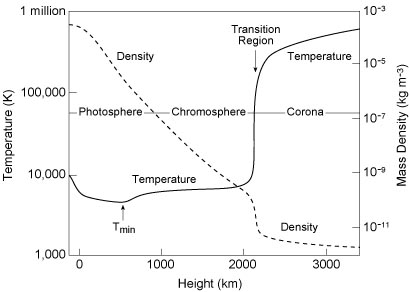
\includegraphics[width=0.45\textwidth]{solar-atm-plot}
  \end{center}
\caption{The temperature of the solar atmosphere decreases from values near 6,000 degrees Kelvin at the visible photosphere to a minimum value of roughly 4,400 degrees Kelvin about 500 kilometers higher up. The temperature increases with height, slowly at first, then extremely rapidly in the narrow transition region, less than 100 kilometers thick, between the chromosphere and corona, from about $10^{4}$K to about $10^{6}$K. (Courtesy of Eugene Avrett, Smithsonian Astrophysical Observatory.) }
\end{wrapfigure}

Through the transition region to the corona and the atmosphere starts to heat considerably to $T\sim10^{7}$K. This region is visible in white light due to Thompson scattering of photospheric light by free electrons and dust in the coronal magnetic field. The plasma beta is less than one through the entire corona meaning magnetic forces dominate and the pressure scale height is approximately $100$Mm.  




%%%%%%%%%%%%Observable Seismic Signatures%%%%%%%%%%%%%%%%%%%%%%%%%%
\subsection{Observable Seismic Signatures}
%Basics of helioseismology and challenges of observing acoustic emission
Helioseismology is a tool for probing the interior of the Sun. Most techniques in this field of analysis rely on observations of gravity and acoustic waves on the photosphere that are the result of interior excitation. Studying the frequency and modes of these oscillations has revealed much about the internal structure of the Sun. Local helioseismology is a collection of techniques developed for global helioseismology that have been modified for use in studying local regions in higher spatial resolution. The following section provides a very basic introduction to some of these techniques. 

\subsubsection{Local Helioseismology}
%use content from old report...maybe expand a little

\paragraph{Helioseismic Holography}\label{helioholog}
\cite{1999ApJ...513L.143D} pioneered the use of helioseismic holography to produce seismic images of the solar flare of July 1996 reported to have a sunquake by Kosovichev and Zharkova. Time series egression-power maps at 3.5 and 6 mHz were computed with a 2 mHz bandwidth. It was found that the most powerful acoustic power frequency associated with the flare is centred at 3.5 mHz but has a large signal to noise ratio. Whereas the 6 mHz range has a much lower ambient noise, therefore producing a better rendering of the seismicity of the flare. It is now standard practice to use the 6 mHz range for helioseismic holographic calculations of egression-power. \\
Originally the idea of analysing Doppler images of the solar surface in order to observe acoustic sources was put forward by \cite{1975CRASB.281...93R}. Helioseismic holography was developed further in concept by Lindsey and Braun \citep{1990SoPh..126..101L, 1992ApJ...392..739B, 1997ApJ...485..895L} in an effort to to image the solar interior and far-side of the Sun. This technique involves using a Doppler image as a representation of the wave-field at a location on the solar surface as a reference point to be able to estimate that wave-field a location in the solar interior at a time preceding or proceeding the image. This is achieved by calculating the ingression or egression of the wave-field by assuming that it's evolution is a, convergence to, or divergence from, the point of origin of that wave-field. 
This technique uses Green's function (eqn \ref{green}, where $\vec{r}$ and $t$ are position and time of an observed signal and $\vec{r}'$ and $t$' are the position and time of the signal earlier in time) which assumes the that the acoustic wave propagates from a point source, allowing a signal $\psi(\vec{r},t)$ observed on the surface to be devolved backwards in time. 

\begin{equation}\label{green}
G_{+}(|\vec{r}-\vec{r}'|,t-t')
\end{equation}

Where $a$ and $b$ constrain the holographic pupil, equation \ref{holog} is then used to devolve the surface signal to calculate the position of subsurface acoustic sources. 

\begin{equation}\label{holog}
H_{+}(\vec{r},z,t)= \int dt'  \int_{a<|\vec{r}-\vec{r}'|<b} d^{2}\vec{r}'G_{+}(|\vec{r}-\vec{r}'|,t-t')\psi(\vec{r}',t')
\end{equation}

Equation \ref{eggpower} is then used to calculate the egression power associated with the acoustic sources at a time $t$. 

\begin{equation}\label{eggpower}
P(z,\vec{r})=\intdt|H_{+}(\vec{r},z,t)|^{2}dt
\end{equation}

If egression power is required in terms of frequency then equation \ref{eggpower} can be Fourier transformed into frequency space.


\paragraph{Time-Distance}\label{TD}
The first observation of a sunquake \citep{1998Natur.393..317K} used the time-distance technique to track sunquake wavefronts. The paper by \cite{1993Natur.362..430D} explains how to extract time-distance (TD) information from observations of intensity fluctuations on the solar surface. This technique uses travel times of waves between two locations on the solar surface. The method assumes that the travel time of a wave propagating in the interior of the Sun will be modified by any anomalies that it has to travel through, thus the resulting signal will contain the signatures of those irregularities. For instance, if the wave encounters a flow along it's path of travel, it will propagate faster with the flow than against it, affecting travel time.     
This technique remaps Dopplergrams into polar coordinates, with the point of origin centered on the area of downflowing material during the flare. This remapped image is then Fourier transformed with respect to azimuthal angle, with the resulting image highlighting cicular disturbances as a line of positive slope.    

%%%%%%%%%%%%%%%%%%%%%%%%%%%MHD of solar flares%%%%%%%%%%%%%%%%%%%%%%%%%%%5
\subsection{Solar Magnetohydrodynamics}\label{MHD}
Most structures observed in the solar atmosphere are a direct result of interplay between plasma and the Sun's dynamic magnetic field. Understanding the relationship between a magnetic field and a plasma is important for describing many observed phenomena. Magnetohydrodynamics (MHD) is a method to determine the continuous macroscopic behaviour of plasma in a magnetic field, thus individual particles are not considered \citep{1982soma.book.....P}. A plasma can be treated as a continuous material if distances between particles are much larger than the mean-free path, or larger than the ion gyro-radius. Where $T$ is plasma temperature, $\lambda_{MFP}$ is mean-free path and $n$ is number of particles in the plasma, equation \ref{meanfreepath} describes the mean-free path. 

\begin{equation}\label{meanfreepath}
\lambda_{MFP}\approx300(\frac{T}{10^{6}K})^{2}(\frac{n}{10^{17}m^{-3}})^{-1}m
\end{equation}

Equation \ref{iongyroradius} is the relationship between particle mass $m$, velocity perpendicular to the magnetic field $v_{\bot}$, charge $q$ and magnetic field strength $B$  which governs the circular motion of a charged particle around a uniform magnetic field or the ion gyro radius. 

\begin{equation}\label{iongyroradius}
r_{g}=\frac{mv_{\bot}}{|q|B}
\end{equation}

In the context of the Sun, and the importance of magnetic fields for processes such as solar flares, MHD builds on the following physical assumptions; a magnetic field can manipulate a plasma by exerting a force on it. Leading to the formation of structure or movement via acceleration; a magnetic field can store the energy required for later release as a solar flare; material wrapped in a magnetic field is thermally protected from it's surroundings; a magnetic field can act as a funnel for plasma and fast particles; and finally, a magnetic field can drive instabilities and support waves \citep{2003dysu.book.....D}.

\subsubsection{MHD Equations}\label{MHDeqns}
Magnetic fields are made up of discreet bundles of magnetic flux known as \emph{flux tubes}. A magnetic flux tube can be thought of as cylindrical in geometry and containing magnetic field lines parallel in orientation to the length of the cylinder. The cross-sectional radius of the tube and magnetic field strength are both variant, magnetic flux contained within the tube however, is constant. Where $\vec{B}$ is magnetic field vector and $\vec{dS}$ is a cross-sectional surface element of the tube, flux $F$ follows the relationship.

\begin{equation}\label{fluxtube}       
F = \int_{S} \vec{B}.\vec{dS}
\end{equation}


The basics of MHD are a built from a combination of Maxwell's electromagnetic equations, material equations, Ohm's law and the fluid dynamics relations. Maxwell's equations and Ohm's law describe electromagnetism in terms of magnetic field $\vec{H}$, magnetic induction $\vec{B}$, magnetic permeability of free space $\mu$, electric field $\vec{E}$, electric displacement $\vec{D}$, electrical permittivity of free space $\epsilon$, charge density $\rho_{c}$ and electric current density $\vec{j}$ 


\begin{equation}\label{max1:ampere}
\nabla\times\vec{H}=\vec{j}+\frac{\partial \vec{D}}{\partial t}
\end{equation}


\begin{equation}\label{max2:faraday}
\nabla\times\vec{E}=-\frac{\partial \vec{B}}{\partial t}
\end{equation}


\begin{equation}\label{max3:gauss}
\nabla\cdot\vec{D}=\rho_{c}
\end{equation}


\begin{equation}\label{max4:nomonopole}
\nabla\cdot\vec{B}=0
\end{equation}

with Ohm's law as,

\begin{equation}\label{ohmslaw}
\vec{E}=\frac{\vec{j}}{\sigma}
\end{equation}

where $\sigma$ is electrical conductivity. The fluid dynamics relations are written in terms of density $\rho$, velocity $\vec{v}$, time $t$, pressure $p$, gas constant $\Re$ and temperature $T$. 
%$\frac{d}{dt}=\frac{\partial}{\partial t}+ \vec{v}\cdot\nabla$, sometimes reffered to as the material derivative, is a way of stating the rate of change with respect to time of the  

\begin{equation}\label{motion}
\rho\frac{d\vec{v}}{dt}=-\nabla p
\end{equation}
 
\begin{equation}\label{masscontinuity}
\frac{d\rho}{dt}+\rho\nabla\cdot\vec{v}=0
\end{equation}

\begin{equation}\label{perfectgaslaw}
p=\Re\rho T
\end{equation}

Equation \ref{motion} is the eqn. of motion describing how the forces are exerted on the fluid are equal to the negative gradient of plasma pressure. Equation \ref{masscontinuity} is the eqn. of mass continuity (mass is conserved), whilst equation \ref{perfectgaslaw} is the perfect gas law relating plasma pressure, density and temperature. The fluid dynamics equations are re-written in terms of MHD by building on the following assumptions: Plasma in a magnetic field experiences the Lorentz force $(\vec{j}\times\vec{B})$, such that a plasma volume element $dV$ carrying a current density $\vec{j}$ per unit volume has the force $\vec{j}dV\times\vec{B}$ exerted on it in a perpendicular direction to the magnetic field. In order to cater for the extra force, equation \ref{motion} has the term $\vec{j}\times\vec{B}$ added to the right hand side.   
Ohm's law states that an electric field in the plasma's frame of reference is proportional to the current, however, the total electric field associated with the movement of plasma is $\vec{E}+\vec{v}\times\vec{B}$ ($\vec{E}$ is the electric field acting on the plasma at rest) therefore, equation \ref{ohmslaw} has the term $\vec{v}\times\vec{B}$ added to it's left hand side.The displacement current term $\frac{\partial \vec{D}}{\partial t}$ in equation \ref{max1:ampere} is neglected due to plasma speeds being much slower than the speed of light.

\subsubsection{Induction Equation}\label{inductioneqn}  
Rewriting equations \ref{max1:ampere}, \ref{max2:faraday} and \ref{ohmslaw} using the assumptions from section \ref{MHDeqns}, with $\nabla\cdot\vec{B} = 0$,

\begin{equation}\label{new1}
\vec{j}=\nabla\times\frac{\vec{B}}{\mu}
\end{equation}

\begin{equation}\label{new2}
\frac{\partial \vec{B}}{\partial t} = - \nabla\times\vec{E}
\end{equation}

\begin{equation}\label{new3}
\vec{E}=-\vec{v}\times\vec{B}+\frac{\vec{j}}{\sigma}
\end{equation}

then substituting \ref{new1} solved for $\vec{j}$ into \ref{new2} we have,

\begin{equation}\label{new4} 
\vec{E}=-\vec{v}\times\vec{B}+\nabla\times\frac{\vec{B}}{\eta} 
\end{equation}

where magnetic diffusivity $=\eta =\frac{1}{\mu\sigma}$.

Substituting \ref{new4}, solved for $\vec{E}$, into \ref{new2},

\begin{equation}\label{new5}
\frac{\partial \vec{B}}{\partial t}=-\nabla\times(-\vec{v}\times\vec{B} + \nabla\times\vec{B}\eta)
                                   =\nabla\times(\vec{v}\times\vec{B})-\nabla\eta\times(\nabla\times\vec{B})
\end{equation}

using the vector identity, $\nabla\times(\nabla\times\vec{A})=\nabla(\nabla\cdot\vec{A})-\nabla^{2}\vec{A}$ the last term in equation \ref{new5} becomes $\nabla(\nabla\cdot\vec{B})-\nabla^{2}\vec{B}$, of which the $\nabla\cdot\vec{B}$ term reduces to zero due to equation \ref{max4:nomonopole}, thus we are left with the induction equation \ref{induction} below. 



\begin{equation}\label{induction}
\frac{\partial \vec{B}}{\partial t}=\nabla\times(\vec{v}\times\vec{B})+\eta\nabla^{2}\vec{B}  
\end{equation}

This equation \ref{induction} can be used to determine $\vec{B}$ if $\vec{v}$ is known. The magnetic Reynolds number,

\begin{equation}\label{reynolds}
R_{m} = \frac{l_{0}v_{0}}{\eta} \sim \frac{\nabla\times(\vec{v}\times\vec{B})}{\eta\nabla^{2}\vec{B}}
\end{equation}

is an approximation of the ratio between the first and second terms on the RHS of the induction equation \ref{induction} if $v_0$ and $l_0$ are typical of the velocity and length-scales over which the system is changing. This ratio can be used to diagnose which part of the induction equation is dominating the MHD of the system. For example if $R_m >> 1$ then the $\nabla\times(\vec{v}\times\vec{B})$ term is large and the second term is negligible, so the induction equation becomes,

\begin{equation}\label{r>>1}
\frac{\partial \vec{B}}{\partial t}=\nabla\times(\vec{v}\times\vec{B}),
\end{equation}

thus induction is dominant and Ohm's law \ref{ohmslaw} becomes $\vec{E} +\vec{v}\times\vec{B}$ meaning the total electric field becomes zero.



If $R_m << 1$ then the $\eta\nabla^{2}\vec{B}$ term is large meaning the induction equation becomes,
\begin{equation}\label{r<<1}
\frac{\partial \vec{B}}{\partial t}=\eta\nabla^{2}\vec{B},
\end{equation}

thus diffusion is dominant so the magnetic field $\vec{B}$ will be varying on a length-scale $L_0$, and so will diffuse with velocity \ref{diffvel}, over the time-scale \ref{difftime}.

\begin{equation}\label{diffvel}
v_d=\frac{L_0}{\tau_d} = \frac{\eta}{L_0}
\end{equation}


\begin{equation}\label{difftime}
\tau_d = \frac{L_{0}^{2}}{\eta}
\end{equation}

%check Foukal pg 125 in the pdf
\citep{2003dysu.book.....D}

%puts .tex file here
%\include{example}
\subsubsection{Plasma Beta}
Another way to write the relationship between $\vec{B}$ and $\vec{v}$ is the equation of motion \ref{motion} modified by the Lorentz force.

\begin{equation}\label{motion1}
\rho\frac{d\vec{v}}{dt}=-\nabla p+\vec{j}\times\vec{B}
\end{equation}

The pressure gradient $-\nabla p$ describes the change from high to low plasma pressure. The Lorentz force, $\vec{j}\times\vec{B}$ acts perpendicularly to the magnetic field, therefore accelerated plasma in a direction parallel to the magnetic field is caused by other forces. If equation \ref{new1} is substituted into the Lorentz force,
\begin{equation}\label{lorentzsub1}
\vec{j}\times\vec{B} = (\nabla\times\frac{\vec{B}}{\mu})\times\vec{B}
\end{equation}

then using the triple vector identity, 
\begin{equation}
\frac{1}2{}\nabla(\vec{B}\cdot\vec{B})=\vec{B}\times(\nabla\times\vec{B})+(\vec{B}\cdot\nabla)\vec{B}
\end{equation}

equation \ref{lorentzsub1} becomes,
\begin{equation}
\vec{j}\times\vec{B} = (\vec{B}\cdot\nabla)\frac{\vec{B}}{\mu}-\nabla(\frac{B^2}{2\mu}) 
\end{equation}

therefore \ref{motion1} becomes:

\begin{equation}\label{maghydstat}
\rho\frac{d\vec{v}}{dt}= -\nabla p + (\vec{B}\cdot\nabla)\frac{\vec{B}}{\mu}-\nabla(\frac{B^2}{2\mu}) 
\end{equation}

Because $-\nabla(\frac{B^2}{2\mu}$ is in the same form as $-\nabla p$ it can be said to be the \emph{magnetic pressure}, providing a force pointing from high to low magnetic pressure as $B^2$ changes with position.A measure of dominance of plasma or magnetic pressure in the motion of plasma is known as the plasma beta, 

\begin{equation}\label{beta}
\beta=\frac{p_{plasma}}{p_mag} = \frac{2p_{0}\mu}{B_{0}^2}
\end{equation}

so if $\beta << 1$ then magnetic pressure is dominant and if $\beta >> 1$ then plasma pressure is dominant.

Another useful relationship to use is pressure scale height, where $g$ is acceleration due to gravity and $T_0$ is uniform temperature, pressure scale height, $H=\frac{P_0}{\rho_{0}g} = \frac{\Re T_{0}}{g}$. When combined with pressure, $p$ for a magneto static plasma with uniform temperature, $p=p_{0}\exp^{\frac{-z}{H}}$, where $z$ is altitude, we have a measure of the height, $H$, over which the pressure of a plasma fall off by a factor of $\exp$. 


\section{Lower Atmospheric Signatures of a Solar Flare Associated with Seismicity}
use old report content + new content in presentation (inc full page plots but better/bigger axis labels)
\begin{itemize}
\item Abstract: Mark didn't like the abstract here
\item Background: Expand and de-itemize background (background should not be covering ground already in previous sections)
\item Observations: More detailed
\item Analysis: David Fanning Ladder plots. Analysis section should include more about techniques used to process the data.
\item Discussion
\item Future Work
\end{itemize}


%%%%%%%%%%%%%%%%%%%%%%%%%%%%%%%%%%%%%%%%%%%%%%%%%%%%%%%%%%%%%%%%%%555
%old report content

\section{Project: Lower Atmospheric Signatures of Solar Flares Associated with Seismicity.}\label{PRJ}
%\begin{abstract}
%Sunquakes represent the propagation of acoustic waves in the sub-photosphere, responding to an excitation of the photosphere during the impulsive phase of solar flares. The progenitors of sunquakes are thought to be either shocks, radiative backwarming, direct particle collision or sudden magnetic field reconfiguration. Each of these mechanisms relies on the transport of energy from the corona to the photosphere, and the physical conditions existing in the chromosphere such as magnetic configuration and density. To understand sunquakes and their relationship to solar flares, we need to understand how energy moves down through the solar atmosphere and the physical conditions that are present. An X1 solar flare with associated sunquake was observed in active region NOAA 12017 on the 29th of March 2014 at 17:46 UTC, by multiple spacecraft, including SDO (HMI), IRIS and RHESSI. Lightcurves of the flare emission from the photosphere, chromosphere and transition region are analysed providing information about the deposition of energy at different altitudes in the solar atmosphere. Hard X-ray footpoints of coronal loops are shown to align well with an area associated with maximum acoustic power. Balmer continuum emission aligned with maximum acoustic power is shown to increase during the flare, indicating the existence of hydrogen recombination continua in the chromosphere possibly leading to radiative backwarming of the photosphere. 
%\end{abstract}

\subsection{Background}
Hard X-ray (HXR) footpoints (1) and UV ribbons (2) observed in the chromosphere directly map to the reconfiguring magnetic fields during the flare: 
1. HXR footpoints are observed due to the excitation of the lower atmosphere by electron particle beams accelerated by the reconnecting magnetic field in the the corona during the flare \citep{1995ApJ...455..347A}.
2.According to the standard flare model \citep{1964NASSP..50..451C, 1966Natur.211..695S, 1974SoPh...34..323H, 1976SoPh...50...85K} magnetic reconnection in the corona leads to energy being directed downward in the form of particles, radiation, MHD waves and conduction of heat, which in turn produces chromospheric ribbons.\\

The majority of the energy released by a flare is deposited in the lower solar atmosphere and manifests itself in the form of enhanced hard X-ray, UV and optical radiation. The production of a sunquake requires a fraction of less than 10-3 of the energy budget available during the flare \citep{2005ApJ...630.1168D}. \\


Optical emission in the lower atmosphere during a flare can occur via two mechanisms \citep{2007ASPC..368..417D}. 
1. Continuum emission from the photosphere is enhanced by heating of the temperature minimum region.
2. Balmer/Paschen continuum emission produced via hydrogen recombination in the chromosphere \\

Balmer/Paschen emission upward (i.e., directly detected) also has a downward component which leads to radiative backwarming of the photosphere \citep{1989SoPh..124..303M}. \\

Sunquakes occur as a result of solar flares depositing energy into the photosphere, stimulating the production of acoustic waves which propagate into the sub-photosphere. These acoustic transients travel into the interior of the sun until they refract back to the surface and are observed as concentric ripples in Dopplergrams \citep{2014arXiv1402.1249K}. \\

The method in which solar flares trigger sunquakes is unknown, although the following mechanisms are thought to be possible progenitors: shocks, radiative backwarming, direct particle collision and sudden magnetic field reconfiguration 



\subsection{Observations}
The X1 flare of the 29th of March 2014 at 17:46 UT in active region NOAA 12017, was observed by SDO, IRIS and RHESSI. HXR data from RHESSI, UV and Balmer emission from IRIS slit-jaw/spectrometer, and visible continuum from SDO HMI are observed during the flare.Balmer emission is taken from IRIS spectroscopic data (wavelength range of 2825.7 and 2825.8Å \citep{2014ApJ...794L..23H}. \\

\begin{figure}\label{saxcontours}
  \begin{center}
  \includegraphics[width=0.40\textwidth]{saxcontours}
  \end{center}
  \caption{From top to bottom shows IRIS Si IV slit-jaw, Mg II slit-jaw and SDO HMI continuum intensity maps.Contours show RHESSI HXR with $E = 25-50$ keV in white or black and HXR with $E = 50-100 keV$ in green, sunspot locations in yellow taken from HMI and 6mHz acoustic power in blue.}
\end{figure}



\subsection{Analysis}
SDO HMI data is subjected to a running difference filter to isolate locations that appear to flare in white light . These enhanced pixels are identified by using a combination of visual inspection and thresholding to eliminate false positives being triggered by noise of similar intensities.Lightcurves are created from SDO HMI continuum processed data. IRIS slit jaw images of Si IV and Mg II are aligned with HMI and lightcurves are created \ref{lcseries} for pixels at the quake and ribbon locations. Lightcurves are created from IRIS spectroscopic data at slit positions aligned with quake and ribbon locations, over a wavelength range within the Balmer continuum. IRIS spectroscopic data are analysed at sunquake, ribbon and non-flaring positions. An egression map of acoustic power is produced  at 6mHz, revealing the position of the sunquake. HXR data from RHESSI and acoustic power data are overlaid on HMI and IRIS slit jaw maps.\\

\begin{figure}\label{lcseries}
  \begin{center} 
\includegraphics[width=0.48\textwidth]{lcseries}
  \end{center}
  \caption{Left panel shows data over the quake location, right panel shows data over the ribbon location. From top to bottom, plots show lightcurves from IRIS Si IV, Mg II and Balmer wavelengths, with the bottom panel showing the lightcurve from SDO HMI. }
\end{figure}

\begin{figure}\label{spectra}
  \begin{center}
  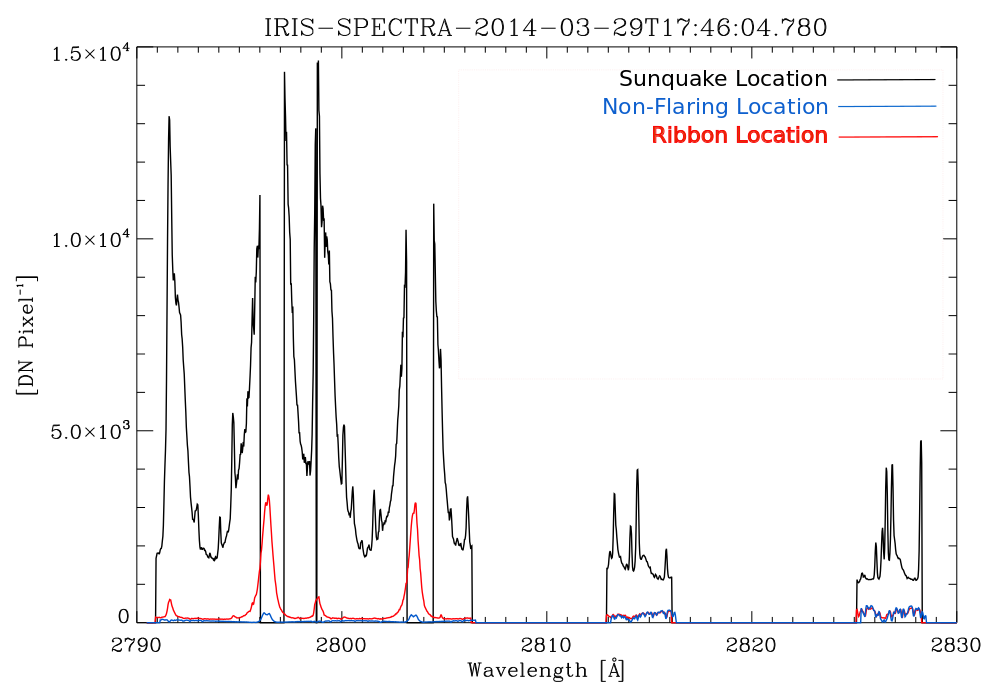
\includegraphics[width=0.58\textwidth]{spectra}
  \end{center}
  \caption{IRIS spectroscopic data ranging in wavelength 2796 - 2830Å with a smaller plot showing a zoom of the region containing the Mg II triplet lines. Black is the spectrum at the quake location (y = 435), red is the spectrum at a point along the ribbon (y = 489) and blue is the spectrum of a non-flaring region (y = 20). Square trough like features represent saturation of the CCD.}
\end{figure}
 

\subsection{First Results and Discussion}
The location of maximum acoustic power, RHESSI HXR, IRIS and SDO intensity correlate both spatially and temporally \ref{saxcontours}, showing that energy input into the upper chromosphere somehow propagates down to the photosphere. Intensity lightcurves \ref{lcseries} from SDO and IRIS seem to suggest a similar representation of the movement of energy through the chromosphere to lower altitudes, since their impulsive appearance and peak intensity occur within a minute of each 
other throughout the different regions. Intensity contrast values shown in \ref{lcseries} give an idea of how much energy is being deposited in each part of the atmosphere but energy calculations are needed. A highly impulsive Balmer continuum \ref{lcseries}, at sunquake and ribbon locations, shows that there is likely to be some radiative backwarming involved in passing energy to the photosphere. Spectroscopic data shown in \ref{spectra} show the sunquake emission to be an order of magnitude greater in amplitude than in the ribbon. The spectrum taken from a non-flaring region is around three orders of magnitude smaller than the sunquake location. Lines over the sunquake location are strongly broadened when compared to spectra elsewhere \ref{spectra}. Ribbon and sunquake spectra appear to be slightly redshifted in comparison to the non-flaring region.\\


\subsection{Future Work}
Calculate energy associated with emission captured by HMI to compare with the acoustic power of the sunquake. Calculate energy associated with emission captured by IRIS slit jaw and spectrometer in order to estimate energy deposition in the atmosphere. Calculate energy associated with Balmer emission to assess likely energy contribution of radiative backwarming. Calculate non-thermal electron power via HXR spectra to estimate the initial energy of the electron beam accelerated by the corona. A more detailed analysis of IRIS spectroscopic data to estimate velocity, density and temperature of chromospheric material. Analysis of triplet lines in the wings of Mg II h \& k will be used to determine heating of the lower chromosphere. Compare spectroscopic data taken by EIS with that of IRIS. Magnetogram: Look at HMI/SOT data to analyse the configuration of the magnetic field.\\

%\appendix
\appendixpage
\addappheadtotoc
%
% \begin{figure}%[H]
%   \begin{center}
%   \includegraphics[width=0.8\textwidth]{}
%   \end{center}
%   \caption{Left panel shows data over the quake location, right panel shows data over the ribbon location. From top to bottom, plots show lightcurves from IRIS Si IV, Mg II, Balmer wavelengths and Mg II wing, with the bottom panel showing the lightcurve from SDO HMI.}\label{lcseries-bold}
% \end{figure}
\section{Ribbon Pixel Coordinates}\label{ribcoords}
%insert figure showing ribbon coords oplot
\begin{figure}%[H]
  \begin{center}
  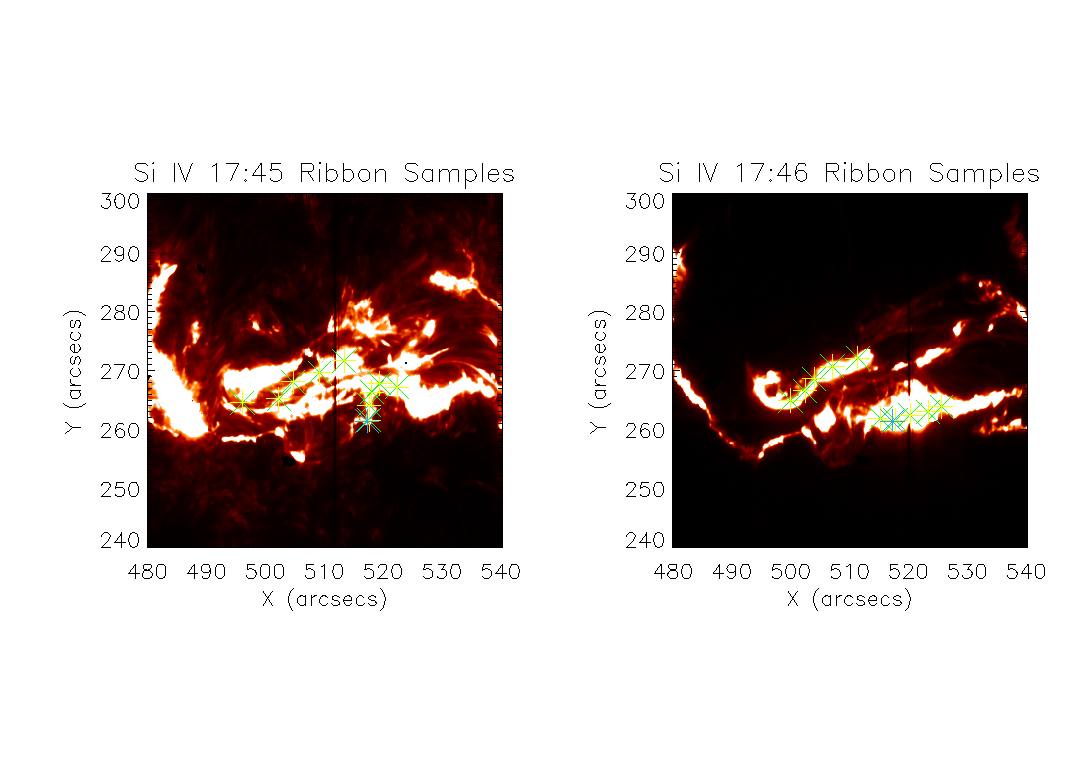
\includegraphics[width=0.8\textwidth]{29-Mar-14-SI-Ribbon-Coord-oplot}
  \end{center}
  \caption{Shows IRIS Si IV slit-jaw data with sampled ribbon and sunquake pixel coordinates marked in green and blue respectively. Twenty ribbon sample points are taken from two instances in time.}\label{sirib}
\end{figure}

\begin{figure}%[H]
  \begin{center}
  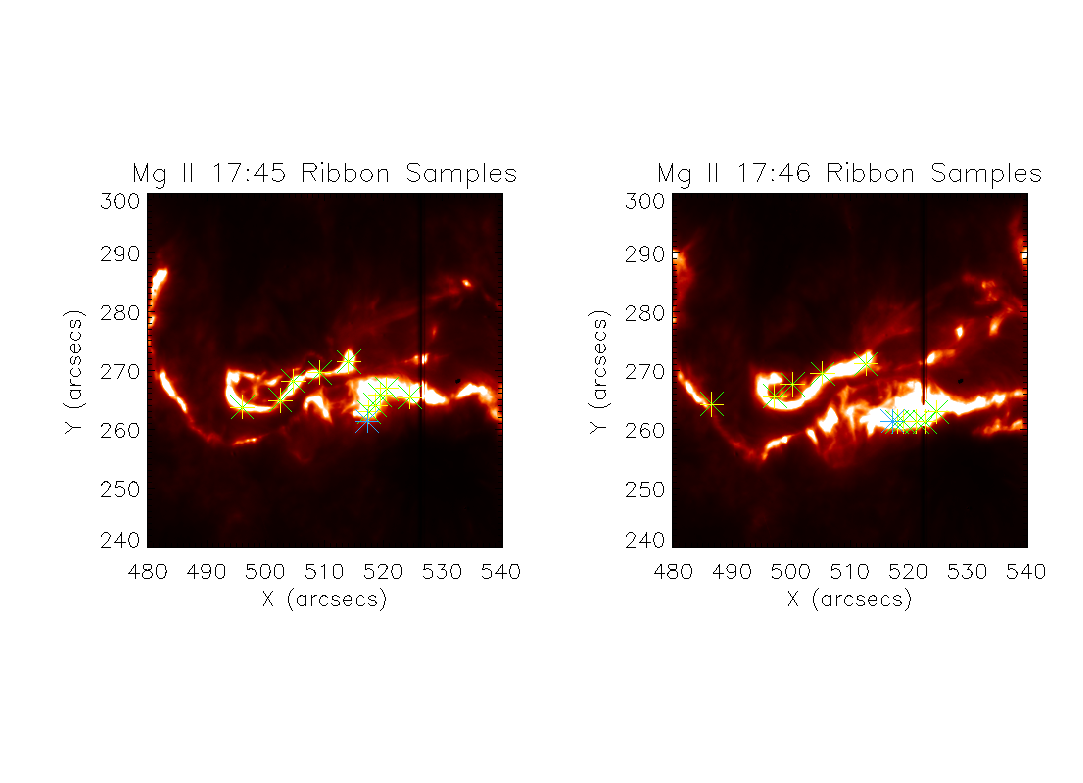
\includegraphics[width=0.8\textwidth]{29-Mar-14-MG-Ribbon-Coord-oplot}
  \end{center}
  \caption{Shows IRIS Mg II slit-jaw data with sampled ribbon and sunquake pixel coordinates marked in green and blue respectively. Twenty ribbon sample points are taken from two instances in time.}\label{mgrib}
\end{figure}

\begin{figure}%[H]
  \begin{center}
  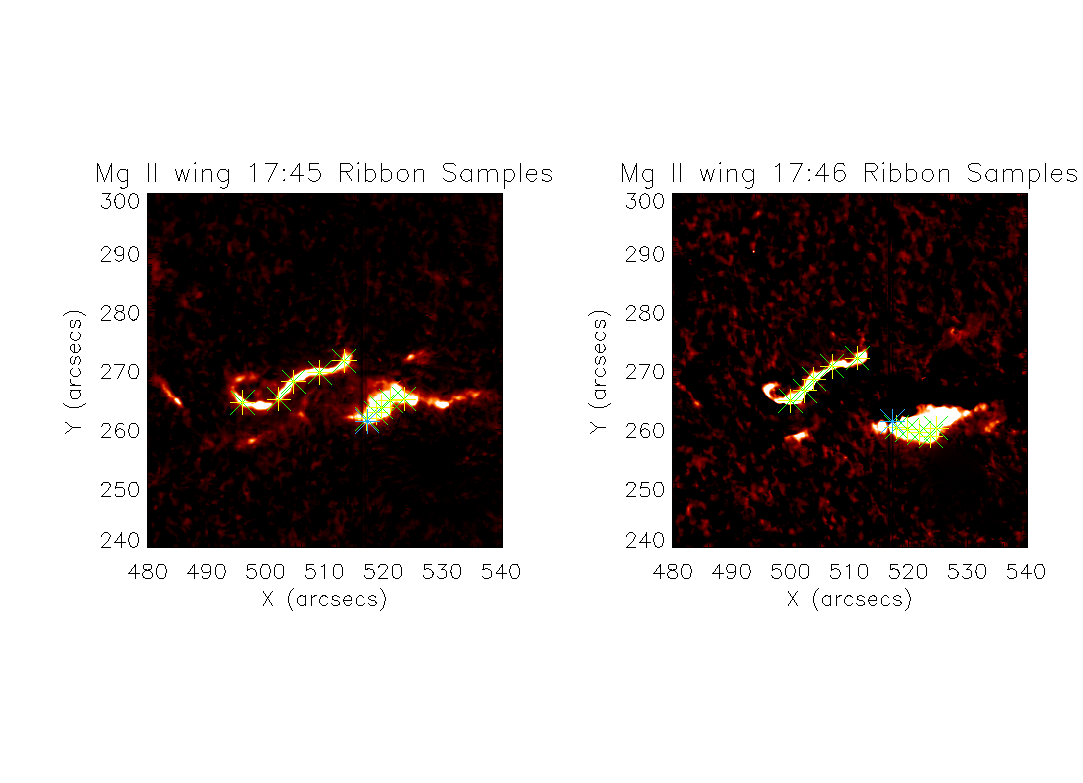
\includegraphics[width=0.8\textwidth]{29-Mar-14-MGW-Ribbon-Coord-oplot}
  \end{center}
  \caption{Shows IRIS Mg II wing slit-jaw data with sampled ribbon and sunquake pixel coordinates marked in green and blue respectively. Twenty ribbon sample points are taken from two instances in time.}\label{mgwrib}
\end{figure}



\label{Bibliography}
\lhead{\emph{Bibliography}}  % Change the left side page header to "Bibliography"
%\bibliographystyle{unsrtnat}  % Use the "unsrtnat" BibTeX style for formatting the Bibliography
\bibliographystyle{plainnat}%abbrv}
\bibliography{../Bibliography/Bibliography}  % The references (bibliography) information are stored in the file named "Bibliography.bib"
%\bibliography{Bibliography}
\end{document}










